% =====================================================================
% IE 643 Course Project — Prep Presentation
% Cross-Template Key-Value Field Extraction from Scanned Forms
%
% Compile on Overleaf with pdfLaTeX. No bibliography backend is needed:
% the reference frames are hand-formatted to the course's mandated
% citation format (instruction 14). refs.bib is kept as a machine-readable
% record for the final report only.
%
% HARD LIMIT: 25 slides (instruction 2). This deck has exactly 25 frames and
% uses no \againframe, no [allowframebreaks] and no pause/overlay splitting,
% so frame count == slide count. VERIFY the last page number in the compiled
% PDF before submitting.
% =====================================================================
\documentclass[aspectratio=169, 11pt]{beamer}

\usetheme{metropolis}
\metroset{progressbar=frametitle, numbering=fraction, block=fill}

\usepackage[utf8]{inputenc}
\usepackage[T1]{fontenc}
\usepackage{booktabs}
\usepackage{array}
\usepackage{tikz}
\usepackage{xcolor}
\usepackage{amsmath}
\usepackage{graphicx}
\usetikzlibrary{arrows.meta, positioning}

\renewcommand{\arraystretch}{1.15}
\definecolor{warn}{HTML}{B3541E}
\definecolor{good}{HTML}{2A7F62}
\definecolor{muted}{HTML}{6C757D}

% NOTE: do not name this \cite — beamer already defines it.
\newcommand{\srcnote}[1]{{\scriptsize\color{muted}[#1]}}
\newcommand{\gap}[1]{{\color{warn}\textbf{#1}}}
% Smaller than \tiny, used only on the three dense reference frames.
\newcommand{\reffont}{\fontsize{4.6}{5.2}\selectfont}

\title{Cross-Template Key-Value Field Extraction from Scanned Forms}
\date{}
\author{}

\begin{document}

% ============================== 1. TITLE =============================
{
\setbeamertemplate{footline}{}
\begin{frame}[plain]
  \vspace{0.2cm}
  {\Large\bfseries Cross-Template Key-Value Field Extraction\\from Scanned Forms\par}
  \vspace{0.15cm}
  {\normalsize\color{muted} Generalizing to Form Templates With Zero Same-Template Training Data\par}
  \vspace{0.4cm}
  \rule{\textwidth}{0.8pt}
  \vspace{0.3cm}

  {\large\bfseries Course Project — IE 643: Deep Learning: Theory and Practice\par}
  \vspace{0.1cm}
  {\normalsize Indian Institute of Technology Bombay\par}
  \vspace{0.45cm}

  \begin{columns}[T]
    \begin{column}{0.52\textwidth}
      {\bfseries Team: Unemployed and Unsupervised}\\[0.25cm]
      \begin{tabular}{@{}ll@{}}
        Param Mehta & \textbf{23b2439}\\
        Arjoe Basak & \textbf{23b1295}\\
      \end{tabular}
    \end{column}
    \begin{column}{0.48\textwidth}
      \footnotesize\color{muted}
      Prep presentation submitted as part of the\\
      IE 643 course project requirement.\\[0.2cm]
      21 September 2026
    \end{column}
  \end{columns}
\end{frame}
}

% ============================= 2. OUTLINE ============================
\begin{frame}{Outline}
  \begin{columns}[T]
    \begin{column}{0.5\textwidth}
      \textbf{1. Problem and Setup}\\
      {\footnotesize\color{muted} The task, and what "zero same-template data" binds us to.}
      \medskip

      \textbf{2. Background Reading}\\
      {\footnotesize\color{muted} Architecture families for document key-value extraction, and what each assumes.}
      \medskip

      \textbf{3. Where the Literature Disagrees}\\
      {\footnotesize\color{muted} Does vision help? Do generative LLMs win? Both unresolved.}
      \medskip

      \textbf{4. Benchmark Integrity}\\
      {\footnotesize\color{muted} Why several standard numbers do not measure what they appear to.}
    \end{column}
    \begin{column}{0.5\textwidth}
      \textbf{5. Datasets and Our Split Protocol}\\
      {\footnotesize\color{muted} What we train on, and how we guarantee no leakage.}
      \medskip

      \textbf{6. Experiments So Far}\\
      {\footnotesize\color{muted} Pipeline validation, and our first seen-vs-unseen gap.}
      \medskip

      \textbf{7. The Gap We Are Addressing}\\
      {\footnotesize\color{muted} Linking has not been measured under template shift.}
      \medskip

      \textbf{8. Roadmap, Risks, References}
    \end{column}
  \end{columns}
\end{frame}

% ========================= 3. PROBLEM STATEMENT ======================
\begin{frame}{The Task}
  \begin{block}{Allotted problem}
    Extract \textbf{key-value fields} from scanned forms, with a representation that
    transfers to form templates the model has \textbf{never seen} — learning from text,
    layout, spatial relationships and field structure on training templates only.
  \end{block}

  \medskip
  \textbf{Why templates break extraction.} A model that scores well on forms of one layout
  has usually learned \emph{where} fields sit, not \emph{what} they are:
  \begin{itemize}
    \item absolute 2D position priors memorise one page geometry;
    \item reading-order serialisation assumes a particular column structure;
    \item "the value is the box to the right of the key" is a template convention, not a rule.
  \end{itemize}

  \medskip
  A genuinely new template invalidates all three at once.
\end{frame}

% ====================== 4. THE ZERO-DATA CONTRACT ====================
\begin{frame}{What "Zero Same-Template Training Data" Binds Us To}
  \begin{columns}[T]
    \begin{column}{0.56\textwidth}
      Held-out templates may not influence training \textbf{in any way}:
      \begin{itemize}
        \item no labelled examples;
        \item \alert{no unlabelled examples} — this rules out most domain-adaptation methods, which assume unlabelled target data is available;
        \item \alert{no validation use} — selecting a checkpoint on a held-out template is leakage even though no gradient flows from it.
      \end{itemize}
      \medskip
      We enforce this in code and print the proof on every run.
    \end{column}
    \begin{column}{0.44\textwidth}
      \scriptsize
      \begin{block}{\scriptsize Emitted by every experiment}
\texttt{LEAKAGE CHECK PASSED [UTL fold 0]}\\
\texttt{~~train templates (2): ['B','C']}\\
\texttt{~~val~~~templates (2): ['B','C']}\\
\texttt{~~test~~templates (1): ['A']}\\
\texttt{~~(train|val) $\cap$ test = []}\\
\texttt{~~no document id in >1 split}
      \end{block}
      {\color{muted} Verified against a negative control that deliberately poisons a split and confirms the assertion fires.}
    \end{column}
  \end{columns}
\end{frame}

% ========================= 5. PIPELINE BACKGROUND ====================
\begin{frame}{Background: The Standard Pipeline}
  \begin{center}
  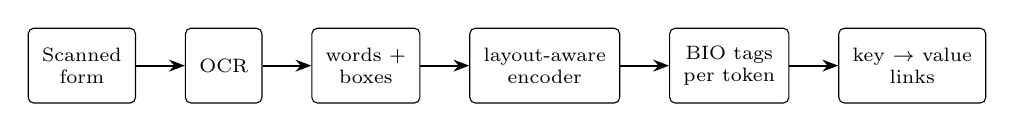
\begin{tikzpicture}[
      node distance=0.5cm and 0.62cm,
      box/.style={draw, rounded corners=2pt, align=center, font=\scriptsize, minimum height=0.95cm, inner xsep=5pt},
      ar/.style={-{Stealth[length=2mm]}, thick}
    ]
    \node[box] (scan) {Scanned\\form};
    \node[box, right=of scan] (ocr) {OCR};
    \node[box, right=of ocr] (tok) {words +\\boxes};
    \node[box, right=of tok] (enc) {layout-aware\\encoder};
    \node[box, right=of enc] (tag) {BIO tags\\per token};
    \node[box, right=of tag] (link) {key $\to$ value\\links};
    \draw[ar] (scan) -- (ocr); \draw[ar] (ocr) -- (tok); \draw[ar] (tok) -- (enc);
    \draw[ar] (enc) -- (tag); \draw[ar] (tag) -- (link);
  \end{tikzpicture}
  \end{center}

  \medskip
  \begin{columns}[T]
    \begin{column}{0.5\textwidth}
      \textbf{Three modalities, jointly}
      \begin{itemize}\small
        \item \textbf{Text} — what the token says
        \item \textbf{Layout} — where it sits (boxes normalised to 0--1000)
        \item \textbf{Vision} — how it looks (rules, shading, boxes)
      \end{itemize}
    \end{column}
    \begin{column}{0.5\textwidth}
      \textbf{Two distinct sub-tasks}
      \begin{itemize}\small
        \item \textbf{Tagging} — per-token classification
        \item \textbf{Linking} — a \emph{relational} problem over entity pairs
      \end{itemize}
      {\small\color{warn} These two are measured under very different conditions in the literature. That becomes the centre of our project.}
    \end{column}
  \end{columns}
\end{frame}

% ==================== 6. FAMILY 1: LAYOUT ENCODERS ===================
\begin{frame}{Family 1 — Layout-Aware Transformer Encoders}
  \small
  \begin{tabular}{@{}lp{4.4cm}p{3.9cm}c@{}}
    \toprule
    \textbf{Model} & \textbf{Position mechanism} & \textbf{Vision stream} & \textbf{FUNSD F1}\\
    \midrule
    LayoutLM & \emph{absolute} 2D position embeddings added to token embeddings & none during pretraining & 78.7 \\
    LayoutLMv2 & spatial-aware self-attention: \emph{relative} $\Delta x,\Delta y$ biases in attention logits & Detectron2 CNN grid, fused early & 82.76 \\
    LayoutLMv3 & relative, plus unified MLM + MIM + word-patch alignment & linear ViT patches, no CNN & \textbf{90.29} \\
    \bottomrule
  \end{tabular}

  \medskip
  \begin{columns}[T]
    \begin{column}{0.52\textwidth}
      \centering
      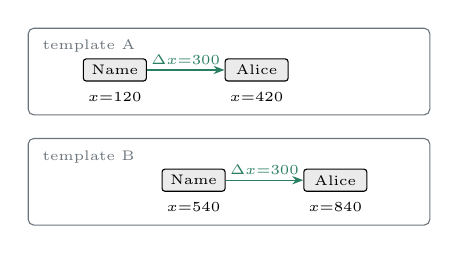
\begin{tikzpicture}[
          tk/.style={draw, fill=black!8, rounded corners=1pt, minimum width=0.8cm,
                     minimum height=0.28cm, font=\tiny, inner sep=1pt},
          ar/.style={-{Stealth[length=1.4mm]}}
        ]
        \draw[muted, rounded corners=2pt] (0,0.45) rectangle (5.1,1.55);
        \node[font=\tiny, muted, anchor=north west] at (0.06,1.52) {template A};
        \node[tk] (k1) at (1.1,1.02) {Name};
        \node[tk] (v1) at (2.9,1.02) {Alice};
        \draw[ar, good] (k1) -- node[above=-1.5pt, font=\tiny, good] {$\Delta x{=}300$} (v1);
        \node[font=\tiny, anchor=north] at (1.1,0.86) {$x{=}120$};
        \node[font=\tiny, anchor=north] at (2.9,0.86) {$x{=}420$};

        \draw[muted, rounded corners=2pt] (0,-0.95) rectangle (5.1,0.15);
        \node[font=\tiny, muted, anchor=north west] at (0.06,0.12) {template B};
        \node[tk] (k2) at (2.1,-0.38) {Name};
        \node[tk] (v2) at (3.9,-0.38) {Alice};
        \draw[ar, good] (k2) -- node[above=-1.5pt, font=\tiny, good] {$\Delta x{=}300$} (v2);
        \node[font=\tiny, anchor=north] at (2.1,-0.54) {$x{=}540$};
        \node[font=\tiny, anchor=north] at (3.9,-0.54) {$x{=}840$};
      \end{tikzpicture}

      \smallskip
      {\tiny\color{warn} Absolute coordinates change with the template. The relative offset does not.}
    \end{column}
    \begin{column}{0.48\textwidth}
      {\footnotesize
      \textbf{The trajectory:} absolute $\to$ relative position encoding, and CNN region
      features $\to$ ViT patches at the same granularity as text tokens.
      \smallskip

      \textbf{Ablation (LayoutLMv3).} MLM+MIM alone 89.19; adding word-patch alignment 89.78.
      {\color{muted} A $+0.59$ gain — real, but small.}}
      \smallskip

      \srcnote{Xu et al., KDD 2020 \textbullet\ Xu et al., ACL 2021 \textbullet\ Huang et al., ACM MM 2022}
    \end{column}
  \end{columns}
\end{frame}

% ================= 7. FAMILY 2: DECOUPLING & RELATIVE ================
\begin{frame}{Family 2 — Decoupling and Relative Encoding}
  \begin{columns}[T]
    \begin{column}{0.5\textwidth}
      \textbf{LiLT} \hfill {\footnotesize MIT}
      \begin{itemize}\footnotesize
        \item Swappable text tower + layout tower, coupled at every layer by \textbf{BiACM}.
        \item Rationale: layout is language-agnostic, so do not let it entangle with one vocabulary.
        \item FUNSD SER F1 \textbf{88.41}; English pretraining transfers to 7 unseen languages on XFUND.
      \end{itemize}
    \end{column}
    \begin{column}{0.5\textwidth}
      \textbf{BROS} \hfill {\footnotesize Apache-2.0}
      \begin{itemize}\footnotesize
        \item \textbf{No visual features at all}; relative 2D encoding gives an attention bias from the offset between box pairs.
        \item \textbf{Area-masked LM} — masks contiguous 2D regions, forcing layout use.
        \item FUNSD F1 \textbf{83.05} — beating LayoutLMv2's 82.76 \emph{with no image}.
      \end{itemize}
    \end{column}
  \end{columns}

  \vspace{0.15cm}
  \begin{center}
  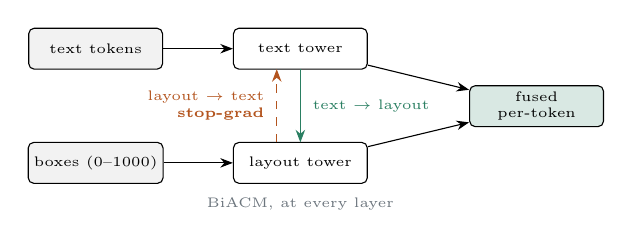
\begin{tikzpicture}[
      b/.style={draw, rounded corners=2pt, align=center, font=\tiny,
                minimum width=1.7cm, minimum height=0.52cm, inner sep=2pt},
      ar/.style={-{Stealth[length=1.6mm]}}
    ]
    \node[b, fill=black!5] (tin) at (0,1.45)  {text tokens};
    \node[b, fill=black!5] (lin) at (0,0)     {boxes (0--1000)};
    \node[b]               (tt)  at (2.6,1.45) {text tower};
    \node[b]               (lt)  at (2.6,0)    {layout tower};
    \node[b, fill=good!18] (out) at (5.6,0.72) {fused\\per-token};

    \draw[ar] (tin) -- (tt);
    \draw[ar] (lin) -- (lt);
    \draw[ar] (tt) -- (out);
    \draw[ar] (lt) -- (out);

    \draw[ar, good]           (2.6,1.19) -- node[right=1pt, font=\tiny, good] {text $\to$ layout} (2.6,0.26);
    \draw[ar, warn, dashed]   (2.3,0.26) -- node[left=1pt, font=\tiny, warn, align=right] {layout $\to$ text\\\textbf{stop-grad}} (2.3,1.19);
    \node[font=\tiny, muted] at (2.6,-0.52) {BiACM, at every layer};
  \end{tikzpicture}
  \end{center}

  \vspace{-0.1cm}
  \srcnote{Wang et al., ACL 2022 \textbullet\ Hong et al., AAAI 2022}
\end{frame}

% ============ 8. FAMILY 3: STRUCTURE BEYOND SEQUENCES ===============
\begin{frame}{Family 3 — Structure Beyond Sequences: Graphs and Parsing}
  \begin{columns}[T]
    \begin{column}{0.53\textwidth}
      \small
      \textbf{The idea.} Linking is \emph{relational}, so model the document as a graph —
      no reading order assumed anywhere.
      \vspace{1pt}

      \begin{center}
      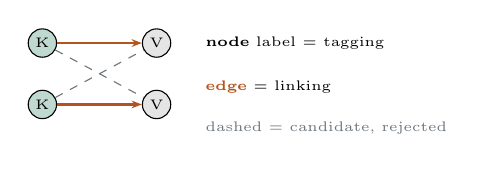
\begin{tikzpicture}[
          n/.style={draw, circle, minimum size=0.36cm, inner sep=0pt, font=\tiny},
          ar/.style={-{Stealth[length=1.3mm]}}
        ]
        \node[n, fill=good!30] (k1) at (0,0.78) {K};
        \node[n, fill=black!10] (v1) at (1.45,0.78) {V};
        \node[n, fill=good!30] (k2) at (0,0) {K};
        \node[n, fill=black!10] (v2) at (1.45,0) {V};
        \draw[muted, dashed] (k1) -- (v2);
        \draw[muted, dashed] (k2) -- (v1);
        \draw[ar, warn, thick] (k1) -- (v1);
        \draw[ar, warn, thick] (k2) -- (v2);
        \node[font=\tiny, anchor=west] at (1.95,0.78) {\textbf{node} label $=$ tagging};
        \node[font=\tiny, anchor=west] at (1.95,0.22) {\textcolor{warn}{\textbf{edge}} $=$ linking};
        \node[font=\tiny, anchor=west, muted] at (1.95,-0.3) {dashed $=$ candidate, rejected};
      \end{tikzpicture}
      \end{center}
      \vspace{1pt}

      {\setlength{\itemsep}{1pt}\setlength{\topsep}{1pt}\setlength{\parsep}{0pt}
      \begin{itemize}\footnotesize
        \item \textbf{SPADE} — extraction as \emph{dependency parsing}; each token points to a parent across multiple graph layers. \gap{+37.3\% relative} linking F1 over serialisation-based baselines.
        \item \textbf{Doc2Graph} — one GNN backbone across form KIE, invoice layout and table detection.
        \item \textbf{PICK} — \emph{learns} a soft adjacency matrix instead of a fixed $k$-NN graph. SROIE 96.12.
        \item \textbf{SDMG-R} — dual-modality fusion; introduced WildReceipt to stress-test unseen templates.
        \item \textbf{FormNet} — \textbf{Rich Attention} (2D distance/direction term in attention) plus \textbf{Super-Tokens} (a GCN pooling spatial neighbours \emph{before} the transformer). V2 adds a multimodal graph-contrastive loss: FUNSD \textbf{86.35}.
      \end{itemize}}
    \end{column}
    \begin{column}{0.47\textwidth}
      \begin{block}{FormNet ablation on FUNSD}
        \small
        {\renewcommand{\arraystretch}{1.0}
        \begin{tabular}{@{}lr@{}}
          \toprule
          Configuration & F1 \\
          \midrule
          ETC baseline & 65.90 \\
          \quad + Rich Attention & 82.22 \\
          \quad + GCN Super-Tokens & 79.37 \\
          \quad + \textbf{both} & \textbf{84.53} \\
          \bottomrule
        \end{tabular}}
      \end{block}
      \vspace{2pt}
      {\footnotesize\color{muted} Structural encoding is worth $+18.6$ F1 over a plain long-sequence transformer — the clearest single piece of evidence that sequence order is the wrong prior for forms.}
      \vspace{2pt}

      {\scriptsize\color{warn}\textbf{Shared weakness.} The graph is built \emph{before} the GNN runs, so bad OCR boxes corrupt everything downstream — a failure mode sequence taggers do not have in the same form.}
    \end{column}
  \end{columns}
\end{frame}

% ================== 9. FAMILY 4: OCR-FREE / GENERATIVE ==============
\begin{frame}{Family 4 — OCR-Free and Generative}
  \begin{columns}[T]
    \begin{column}{0.5\textwidth}
      \small
      \textbf{Donut} — Swin encoder $\to$ BART decoder generates structured JSON directly.
      No OCR, no boxes, no graph: extraction and linking collapse into one decode.
      \smallskip

      \textbf{DocLLM} — disentangles self-attention into four matrices (text$\to$text,
      text$\to$spatial, spatial$\to$text, spatial$\to$spatial). No vision encoder; boxes only.
      \smallskip

      \textbf{Identify, Locate, Link} (ICDAR 2026) — a 256M-parameter VLM doing identify +
      locate + link in a single generative pass, with native \textbf{many-to-many} key-value
      relations and a layout-aware evaluation metric.
    \end{column}
    \begin{column}{0.5\textwidth}
      \begin{alertblock}{The cost of going generative}
        \small
        DocLLM's own reported numbers:
        \smallskip

        \begin{tabular}{@{}lr@{}}
          FUNSD & \gap{51.8} \\
          CORD & 67.4 \\
          SROIE & 91.9 \\
        \end{tabular}
        \smallskip

        Against 83--93 on FUNSD for BROS, LayoutLMv3 and GeoLayoutLM — despite far more parameters.
      \end{alertblock}
      {\footnotesize\color{muted}
      Free-form generation does not structurally guarantee well-formed spans the way a tagging or graph head does.}
    \end{column}
  \end{columns}
\end{frame}

% =================== 10. CONFLICTING FINDINGS ========================
\begin{frame}{Where the Literature Disagrees}
  \begin{columns}[T]
    \begin{column}{0.5\textwidth}
      \begin{block}{Does the vision stream help?}
        \small
        \textbf{Against:} BROS reaches 83.05 on FUNSD with \emph{no image}, beating
        LayoutLMv2's 82.76 \emph{with} one. Its claim: serialisation errors, not missing
        vision, were the real bottleneck.
        \smallskip

        \textbf{For:} LayoutLMv3, DocFormerv2 and FormNetV2 all show gains — but only when
        vision is fused at \emph{token} or \emph{relation} granularity, not page-wide.
        \smallskip

        \textbf{Unresolved:} no controlled ablation exists holding backbone size, pretraining
        corpus and architecture fixed.
      \end{block}
    \end{column}
    \begin{column}{0.5\textwidth}
      \begin{block}{Do generative LLMs win?}
        \small
        \textbf{For:} LMDX drops \gap{$<$5 F1} from seen to unseen templates on VRDU, where
        LayoutLMv2 drops \gap{19--27}.
        \smallskip

        \textbf{Against:} DocLLM scores 51.8 on FUNSD, far below discriminative encoders.
        \smallskip

        \textbf{Reading both:} generative models may generalise better across templates while
        being worse at exact span boundaries. These are different quantities — and the two
        claims have never been tested in one experiment.
      \end{block}
    \end{column}
  \end{columns}
\end{frame}

% ================= 11. MEASURED EVIDENCE ON SHIFT ====================
\begin{frame}{What Is Actually \emph{Measured} About Template Shift}
  \footnotesize
  \begin{columns}[T]
    \begin{column}{0.48\textwidth}
      \textbf{1. The gap is real and large.}\\
      VRDU, Registration Forms, 200 training documents:
      \vspace{2pt}

      {\renewcommand{\arraystretch}{1.0}
      \begin{tabular}{@{}lrr@{}}
        \toprule
        & Seen (MTL) & Unseen (UTL)\\
        \midrule
        FormNet & 90.51 & \gap{77.29}\\
        \bottomrule
      \end{tabular}}
      \vspace{2pt}

      A \gap{13.22-point} gap; 13--17 points across models.
      \smallskip

      \textbf{2. Relative encoding is no guarantee.}\\
      MIDV2020, unseen-template country split:
      \vspace{2pt}

      {\renewcommand{\arraystretch}{1.0}
      \begin{tabular}{@{}lr@{}}
        \toprule
        KNN-Former & 87.88\\
        LayoutLM-base & 47.65\\
        \textbf{BROS} & \gap{23.31}\\
        \bottomrule
      \end{tabular}}
      \vspace{2pt}

      {\color{warn} BROS degrades \emph{worst}, despite being designed around relative position encoding.}
    \end{column}
    \begin{column}{0.48\textwidth}
      \textbf{3. "Unseen template" is not mainly geometry.}\\
      Do-GOOD decomposes the shift for LayoutLMv3 on FUNSD (in-distribution 90.29):
      \vspace{2pt}

      {\renewcommand{\arraystretch}{1.0}
      \begin{tabular}{@{}lrr@{}}
        \toprule
        Shift type & F1 & Drop\\
        \midrule
        Text only & 86.82 & 3.47\\
        \textbf{Layout only} & 84.95 & \textbf{5.34}\\
        Human-intervened & 73.25 & 17.04\\
        \textbf{Real-world} & 57.88 & \gap{32.41}\\
        \bottomrule
      \end{tabular}}
      \vspace{2pt}

      \begin{alertblock}{\footnotesize Design consequence}
        \scriptsize Pure layout novelty is the \emph{smallest} component. Optimising only the
        positional encoding targets 5 points of a 32-point problem.
      \end{alertblock}
    \end{column}
  \end{columns}
\end{frame}

% =================== 12. BENCHMARK INTEGRITY =========================
\begin{frame}{Benchmark Integrity — Which Numbers Mean Anything}
  \small
  \begin{block}{Template leakage inside standard benchmarks}
    Measured train/test template duplication: \textbf{SROIE \gap{75\%}}, \textbf{FUNSD 16\%}.
    Most published SROIE "generalization" numbers are not measuring cross-template
    performance at all. \srcnote{Laatiri et al., ICDAR 2023}
  \end{block}

  \begin{block}{FUNSD's annotation leaks entity boundaries}
    Block-level annotation gives every token inside an entity \emph{identical} coordinates, so
    models learn "block boundary = entity boundary" rather than semantics. Re-annotating
    entity-centrically (EC-FUNSD) drops scores markedly. \srcnote{Zhang et al., 2024}
  \end{block}

  \begin{block}{FUNSD's linking ground truth is too noisy to benchmark}
    PEneo re-annotated FUNSD and XFUND into \textbf{RFUND} precisely because the originals
    were inadequate for key-value pair evaluation. \srcnote{Lin et al., ACM MM 2024}
  \end{block}

  \medskip
  \centering{\color{warn}\textbf{Consequence for us: FUNSD validates our \emph{code}. It cannot validate our \emph{claim}.}}
\end{frame}

% ======================= 13. DATASET SURVEY ==========================
\begin{frame}{Dataset Survey}
  \scriptsize
  \begin{tabular}{@{}lrccp{3.3cm}@{}}
    \toprule
    \textbf{Dataset} & \textbf{Docs} & \textbf{Many templates?} & \textbf{KV linking?} & \textbf{Official unseen-template split?}\\
    \midrule
    \textbf{VRDU} Registration & 1,915 & 3 & no & \textcolor{good}{\textbf{yes} — STL/MTL/UTL}\\
    \textbf{VRDU} Ad-buy & 641 & dozens & no & \textcolor{good}{\textbf{yes} — STL/MTL/UTL}\\
    \textbf{DocILE} & 6.7k + 100k synth & many & no (KILE + line items) & \textcolor{good}{yes} — 0-/few-/many-shot layouts\\
    \textbf{FUNSD} & 199 & yes, unlabelled & \textcolor{good}{\textbf{yes}} & no\\
    \textbf{XFUND} & 1,393 & yes, unlabelled & \textcolor{good}{\textbf{yes}} & no (7 languages)\\
    \textbf{KVP10k} & 10,707 & yes & \textcolor{good}{\textbf{yes}, open-set keys} & no\\
    \textbf{CORD} & 1,000 & receipts & no & no\\
    \textbf{SROIE} & 1,000 & \textcolor{warn}{75\% duplicated} & no & no\\
    \bottomrule
  \end{tabular}

  \smallskip
  \begin{alertblock}{The structural problem}
    \footnotesize The dataset with an official unseen-template protocol (\textbf{VRDU}) has \textbf{no
    linking annotation}. The datasets with linking annotation (\textbf{FUNSD}, \textbf{XFUND},
    \textbf{KVP10k}) have \textbf{no template split}. This is the shape of the field, not an
    oversight in our search — and it is what makes our question worth asking.
  \end{alertblock}
\end{frame}

% ====================== 14. CHOSEN DATASETS ==========================
\begin{frame}{Datasets We Will Use, and Why}
  \begin{columns}[T]
    \begin{column}{0.5\textwidth}
      \textbf{Primary — VRDU}\\
      {\footnotesize The only ready-made Unseen Template Learning protocol. Registration Forms
      (3 templates) to establish the method; Ad-buy Forms (dozens) to reach $\geq$4 training and
      $\geq$2 held-out templates. Its published 13--17 point gap calibrates ours.}
      \medskip

      \textbf{Secondary — FUNSD via RFUND}\\
      {\footnotesize Carries the key$\to$value links VRDU lacks. Used for the \emph{linking} half,
      with RFUND's corrected annotation, and never as generalization evidence on its own.}
    \end{column}
    \begin{column}{0.5\textwidth}
      \textbf{Our own curation — synthetic templates}\\
      {\footnotesize Real blank fillable PDFs (CommonForms, $\sim$55k; IRS W-2/1040/W-9)
      $\to$ fill AcroForm widgets with Faker values via PyMuPDF $\to$ log each widget's box,
      label and link as \emph{exact} ground truth $\to$ degrade with Augraphy to look scanned.}
      \medskip

      {\footnotesize\textbf{Why this matters:} it is the only route that \emph{guarantees} zero
      leakage. Any scraped corpus can contain incidental template overlap we cannot rule out.}
    \end{column}
  \end{columns}

  \medskip
  {\footnotesize\color{muted}
  Considered and deferred: \textbf{DocILE} — better designed for this question, but token-gated
  access and Line Item Recognition add table modelling beyond our current scope.}
\end{frame}

% ====================== 15. SPLIT PROTOCOL ===========================
\begin{frame}{Our Split Protocol}
  \begin{center}
  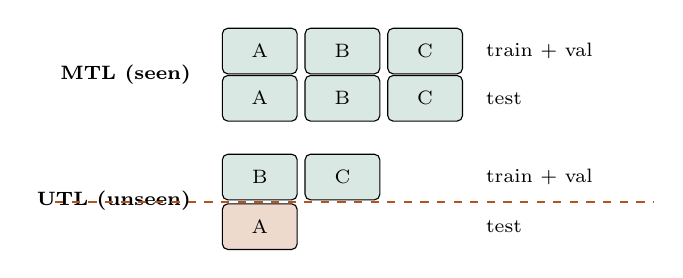
\begin{tikzpicture}[
      t/.style={draw, rounded corners=2pt, minimum width=0.95cm, minimum height=0.58cm, font=\scriptsize}
    ]
    \node[font=\scriptsize\bfseries, anchor=east] at (-0.75, 0.88) {MTL (seen)};
    \foreach \i/\x in {A/0, B/1.05, C/2.1} {
      \node[t, fill=good!18] at (\x, 1.18) {\i};
      \node[t, fill=good!18] at (\x, 0.58) {\i};
    }
    \node[font=\scriptsize, anchor=west] at (2.75, 1.18) {train + val};
    \node[font=\scriptsize, anchor=west] at (2.75, 0.58) {test};

    \node[font=\scriptsize\bfseries, anchor=east] at (-0.75, -0.72) {UTL (unseen)};
    \foreach \i/\x in {B/0, C/1.05} { \node[t, fill=good!18] at (\x, -0.42) {\i}; }
    \node[t, fill=warn!22] at (0, -1.05) {A};
    \node[font=\scriptsize, anchor=west] at (2.75, -0.42) {train + val};
    \node[font=\scriptsize, anchor=west] at (2.75, -1.05) {test};

    \draw[dashed, thick, warn] (-2.6, -0.74) -- (5.0, -0.74);
  \end{tikzpicture}
  \end{center}

  \medskip
  \begin{columns}[T]
    \begin{column}{0.56\textwidth}
      \small
      \begin{itemize}
        \item \textbf{Leave-one-template-out}, one fold per template.
        \item \textbf{Matched training-set size} across regimes — otherwise the "gap" is really a sample-efficiency curve.
        \item $\geq$3 seeds; report mean $\pm$ standard deviation.
      \end{itemize}
    \end{column}
    \begin{column}{0.44\textwidth}
      \small
      \[ \text{gap} = \overline{F_1^{\,\text{MTL}}} - \overline{F_1^{\,\text{UTL}}} \]
      {\footnotesize\color{muted} Our implementation raises an error rather than reporting a gap
      if the two regimes end up with different training-set sizes.}
    \end{column}
  \end{columns}
\end{frame}

% =================== 16. DATA CURATION ROADMAP =======================
\begin{frame}{Data Curation Pipeline}
  \begin{center}
  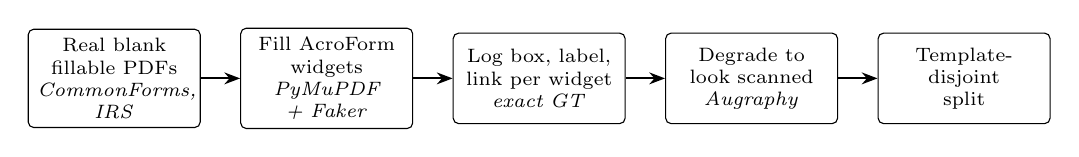
\begin{tikzpicture}[
      node distance=0.45cm and 0.5cm,
      box/.style={draw, rounded corners=2pt, align=center, font=\scriptsize, minimum height=1.15cm, text width=1.95cm},
      ar/.style={-{Stealth[length=2mm]}, thick}
    ]
    \node[box] (a) {Real blank\\fillable PDFs\\\textit{CommonForms, IRS}};
    \node[box, right=of a] (b) {Fill AcroForm\\widgets\\\textit{PyMuPDF + Faker}};
    \node[box, right=of b] (c) {Log box, label,\\link per widget\\\textit{exact GT}};
    \node[box, right=of c] (d) {Degrade to\\look scanned\\\textit{Augraphy}};
    \node[box, right=of d] (e) {Template-\\disjoint\\split};
    \draw[ar] (a) -- (b); \draw[ar] (b) -- (c); \draw[ar] (c) -- (d); \draw[ar] (d) -- (e);
  \end{tikzpicture}
  \end{center}

  \medskip
  \begin{columns}[T]
    \begin{column}{0.5\textwidth}
      \textbf{Why this earns its cost}
      \begin{itemize}\small
        \item Ground truth is free and exact — we wrote the values in.
        \item Template identity is known by construction, not inferred by clustering.
        \item Lets us vary \emph{one} factor at a time: same template, different degradation — isolating layout novelty from scan noise, which is exactly the Do-GOOD decomposition.
      \end{itemize}
    \end{column}
    \begin{column}{0.5\textwidth}
      \textbf{Open risk}
      \smallskip

      {\footnotesize Whether synthetic template diversity actually improves generalization to
      \emph{real} unseen templates is, as far as our review found, \textbf{not cleanly measured
      anywhere in the literature}. We treat it as a hypothesis to test, not an assumption to
      build on.}
    \end{column}
  \end{columns}
\end{frame}

% ============ 17. METRICS, TAXONOMY AND DIAGNOSTICS ==================
\begin{frame}{Metrics, Failure Taxonomy and Early Diagnostics}
  \begin{columns}[T]
    \begin{column}{0.52\textwidth}
      \textbf{Metrics}
      \begin{itemize}\scriptsize
        \item \textbf{Entity F1} — strict IOB2, exact span and type via \texttt{seqeval}. Dual-implementation cross-check passed ($\Delta=0.00$).
        \item \textbf{Gap} — $\overline{F_1^{\,\text{MTL}}} - \overline{F_1^{\,\text{UTL}}}$, matched size ($n=200$), 3 seeds.
      \end{itemize}
      \smallskip

      \textbf{Four failure buckets (instrumented)}
      \begin{enumerate}\scriptsize
        \item \textbf{OCR / recognition} — wrong characters (\textbf{0.2\%})
        \item \textbf{Layout association} — right text, wrong key (\textbf{1.1\%})
        \item \textbf{Field type schema} — right place, wrong label (\textbf{97.2\%})
        \item \textbf{Repeated structure} — line items split/merged (\textbf{1.5\%})
      \end{enumerate}
      \smallskip

      {\tiny\color{muted} Diagnostics: Malformed \texttt{I-} tags ($2.3\%$), length truncation count.}
    \end{column}
    \begin{column}{0.48\textwidth}
      \centering
      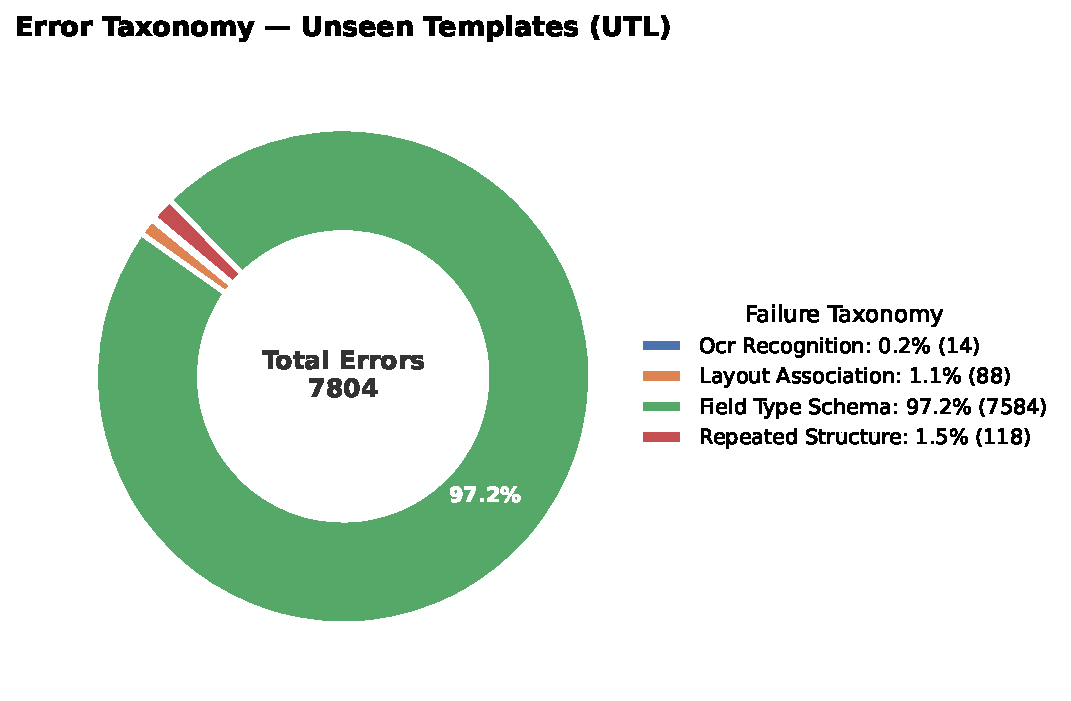
\includegraphics[width=\linewidth]{figures/error_taxonomy.pdf}
      \vspace{-0.15cm}

      {\scriptsize\textbf{Pilot finding on UTL:} Schema/type misalignment accounts for 97.2\% of errors; OCR corruption is negligible (0.2\%). Failure is purely structural.}
    \end{column}
  \end{columns}
\end{frame}

% ================== 18. EXPERIMENT 1: PIPELINE =======================
\begin{frame}{Experiment 1 — Pipeline Validation (FUNSD)}
  \begin{columns}[T]
    \begin{column}{0.48\textwidth}
      {\footnotesize\textbf{Setup \& Purpose.} LiLT (\texttt{lilt-roberta-en-base}, MIT), FUNSD 149/50 split, 3 seeds. Validates 0--1000 box normalisation, subword alignment, and strict IOB2 metric before trusting cross-template gaps.}
      \vspace{0.2cm}

      \begin{block}{Result (3 seeds, mean $\pm$ std)}
        \centering\footnotesize
        \textbf{Entity F1 = 0.7929 $\pm$ 0.0136}\\
        {\scriptsize Seeds: 13 $\to$ 0.7779 \quad 21 $\to$ 0.7961 \quad 42 $\to$ 0.8046}\\[0.05cm]
        {\tiny Cross-check: $\Delta=0.00$ (seqeval == independent) $\mid$ Malformed $I\text{-}$: 2.3\%}
      \end{block}
    \end{column}
    \begin{column}{0.52\textwidth}
      \centering
      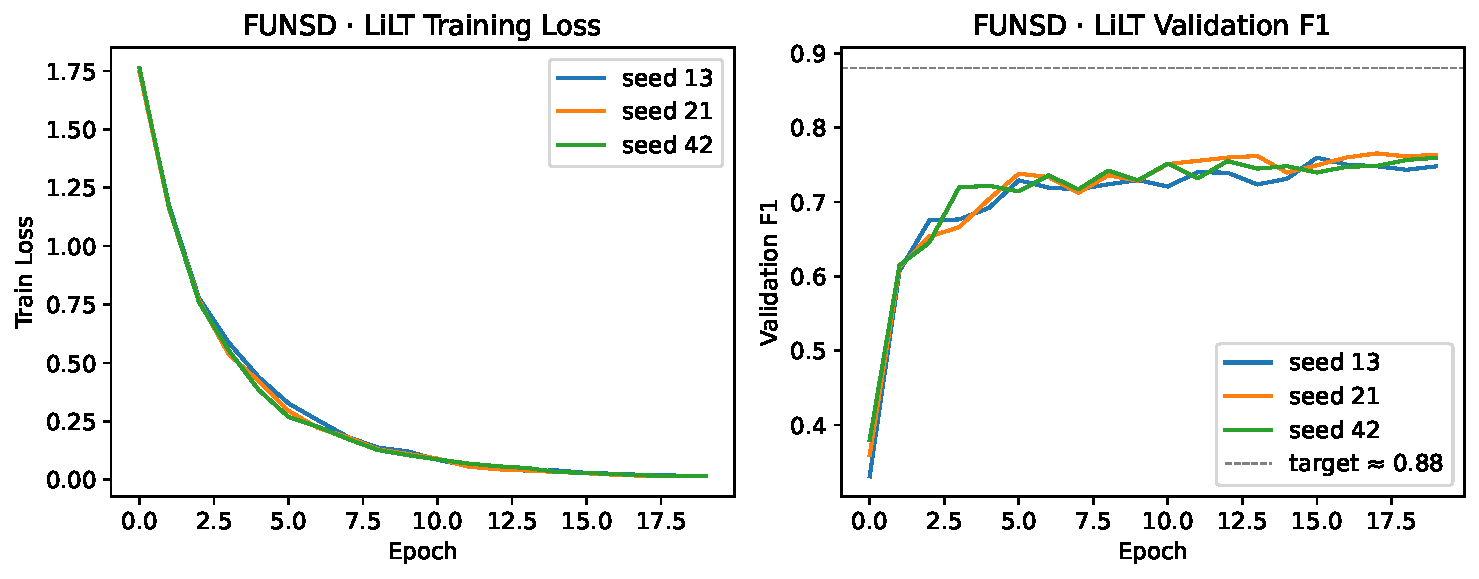
\includegraphics[width=\linewidth]{figures/funsd_curve.pdf}
      \vspace{0.1cm}

      \begin{alertblock}{Read this number correctly}
        \scriptsize
        \gap{Gate not met.} We pre-registered ``within a couple of points of the published 88.41''.
        We are \gap{9 points short}. Metric strictness is \emph{excluded} (lenient IOB2 scores
        \emph{lower}: 0.7614/0.7793/0.7891). Open suspects: training length, and HEADER collapsing
        to 0.50 F1. \textbf{Fixing this is our next action.}
      \end{alertblock}
    \end{column}
  \end{columns}
\end{frame}

% ================== 19. EXPERIMENT 2: THE GAP ========================
\begin{frame}{Experiment 2 — Seen vs.\ Unseen Templates (VRDU)}
  \begin{columns}[T]
    \begin{column}{0.48\textwidth}
      {\footnotesize\textbf{Setup.} VRDU Registration Forms, leave-one-template-out (3 folds $\times$ 3 seeds $=$ 9 runs \emph{per regime}, 18 in total), matched size ($n=200$). Leakage check: 0 test templates in train.}
      \vspace{0.2cm}

      \begin{block}{Result (matched $n=200$, 9 runs per regime)}
        \scriptsize
        \begin{tabular}{@{}lr@{}}
          \toprule
          Seen (MTL), mean F1 & \textbf{0.8774} $\pm$ 0.0162\\
          Unseen (UTL), mean F1 & \textbf{0.6666} $\pm$ 0.0729\\
          \midrule
          \textbf{Generalization Gap ($\Delta$)} & \gap{$-$0.2108} ($-$21.1 pts)\\
          Relative performance drop & \gap{$-$24.03\%}\\
          \bottomrule
        \end{tabular}
      \end{block}
    \end{column}
    \begin{column}{0.52\textwidth}
      \centering
      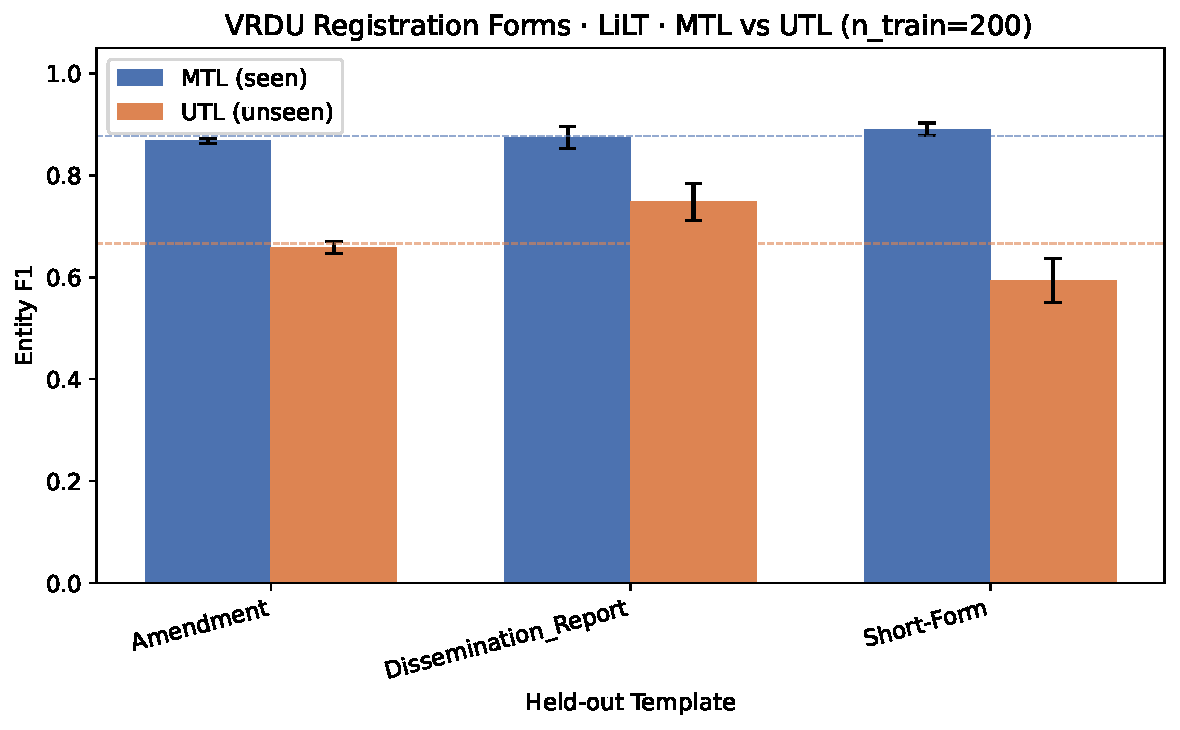
\includegraphics[width=0.88\linewidth]{figures/vrdu_gap.pdf}
      \vspace{-0.2cm}

      {\scriptsize\textbf{Key Finding:} Form-Short drops steepest ($0.88 \to 0.58$); degradation is consistent across folds.\\[0.05cm]
      \textbf{Validity:} both regimes share identical code, data handling and metric, so the
      \emph{gap} is a sound within-study comparison even though Slide 18's absolute level is low.
      We therefore do \emph{not} yet set our 21.1 pts against FormNet's 13.2 ($90.5 \to 77.3$) —
      a depressed baseline inflates a gap. That comparison waits on the Slide 18 fix.}
    \end{column}
  \end{columns}
\end{frame}

% ====================== 20. THE GAP WE CLAIM =========================
\begin{frame}{The Research Gap We Are Addressing}
  \footnotesize
  {\color{warn}\textbf{Observation from our review.}} Entity extraction \emph{has} been measured
  under template shift — VRDU, DocILE and Do-GOOD all do it. Key-value \textbf{linking} has not.
  Every strong linking number we found comes from a split where train and test share templates.

  \vspace{1pt}
  \scriptsize
  {\renewcommand{\arraystretch}{0.95}
  \begin{tabular}{@{}>{\raggedright\arraybackslash}p{2.4cm}>{\raggedright\arraybackslash}p{5.3cm}>{\raggedright\arraybackslash}p{4.6cm}@{}}
    \toprule
    \textbf{Work} & \textbf{Linking result} & \textbf{Split}\\
    \midrule
    GeoLayoutLM & FUNSD RE F1 80.35 $\to$ \textbf{89.45} & same-template \\
    BROS (SPADE-EL) & FUNSD entity linking & same-template \\
    KVPFormer & +7.2\% FUNSD, +13.2\% XFUND & same-template \\
    PEneo & +19.9--22.9\% on RFUND-EN & same-template \\
    ZeroShotCeres & zero-shot relations, unseen templates & \textcolor{good}{template-disjoint} — but \textbf{webpages}\\
    Majumder et al. & unseen invoice templates & \textcolor{good}{template-disjoint} — but \textbf{field typing}, not linking\\
    \bottomrule
  \end{tabular}}

  \vspace{1pt}
  \footnotesize\centering\textbf{Our contribution: measure tagging \emph{and} linking under one template-disjoint protocol.}\\
  {\scriptsize\color{muted} Stated as "to our knowledge" — we have not exhaustively verified DocILE's task structure.}
\end{frame}

% ======================== 21. ROADMAP ================================
\begin{frame}{Future Plan of Action — Subtasks and Roadmap}
  \renewcommand{\arraystretch}{1.05}
  \scriptsize
  \centering
  \begin{tabular}{@{}clp{9.0cm}c@{}}
    \toprule
    & \textbf{Subtask} & \textbf{Content} & \textbf{Owner}\\
    \midrule
    \textcolor{good}{\textbf{done}} & S0 Pipeline & Loaders, split + leakage assertion, dual metric implementation & both\\
    \textcolor{good}{\textbf{done}} & S1 VRDU loader & Parse VRDU to words/boxes/tags with template ids & PM\\
    \textcolor{good}{\textbf{done}} & S2 Gap measurement & MTL vs UTL, matched size, 3 seeds ($\Delta = 21.1$ pt gap verified) & PM\\
    3 & S3 Linking head & BROS SPADE-EL on RFUND; linking F1 under holdout & AB\\
    4 & S4 Scale up & VRDU Ad-buy: $\geq$4 training, $\geq$2 held-out templates & AB\\
    5 & S5 Synthetic templates & CommonForms + PyMuPDF + Augraphy & AB\\
    6 & S6 Ablations & Absolute vs relative position, $\pm$vision, OCR-free, reading order & PM\\
    \textcolor{good}{\textbf{done}} & S7 Failure analysis & Per-template, per-bucket error breakdown (taxonomised on UTL) & both\\
    8 & S8 Interface & Gradio upload $\to$ highlighted key-value boxes & PM\\
    9 & S9 Report & Stage-wise report & both\\
    \bottomrule
  \end{tabular}
\end{frame}

% ==================== 22. MODELS, DEMO, RISKS ========================
\begin{frame}{Models Under Investigation, Interface, and Risks}
  \begin{columns}[T]
    \begin{column}{0.48\textwidth}
      \textbf{Models and licences}
      \smallskip

      \scriptsize
      \begin{tabular}{@{}>{\raggedright\arraybackslash}p{2.3cm}l>{\raggedright\arraybackslash}p{2.0cm}@{}}
        \toprule
        Model & Licence & Role\\
        \midrule
        LiLT & MIT & primary\\
        LayoutLMv3 & \textcolor{warn}{CC-BY-NC-SA} & strong baseline\\
        BROS & Apache-2.0 & linking head\\
        Qwen2.5-VL-7B-Instruct & Apache-2.0 & zero-shot baseline\\
        \bottomrule
      \end{tabular}
      \smallskip

      {\footnotesize All are pretrained on IIT-CDIP ($\sim$11M scanned pages) except the VLM.
      LayoutLMv3's licence is \textbf{non-commercial} — acceptable for coursework, and declared here.
      \smallskip

      \textbf{Still to investigate:} GeoLayoutLM (best published linking F1), UDOP, SmolDocling.}
    \end{column}
    \begin{column}{0.48\textwidth}
      \textbf{Interface}\\
      {\footnotesize Gradio \texttt{AnnotatedImage}: upload a form, see predicted key-value pairs
      highlighted on the page with per-field confidence.}
      \smallskip

      \textbf{Risks and mitigations}
      \scriptsize
      \begin{tabular}{@{}p{2.2cm}p{3.0cm}@{}}
        \toprule
        Risk & Mitigation\\
        \midrule
        Only 3 templates in VRDU Registration & Move to Ad-buy; add synthetic families\\
        Gap is seed noise & $\geq$3 seeds, report std\\
        Kaggle GPU quota & LiLT is small; 30 h/week suffices\\
        Unverified citations & Flagged in the repo; primary-source check before the report\\
        \bottomrule
      \end{tabular}
    \end{column}
  \end{columns}
\end{frame}

% ==================== 23-25. REFERENCES ==============================
\begin{frame}{References — Benchmarks, Datasets and Benchmark Integrity}
  \reffont
  {\setlength{\itemsep}{0pt}\setlength{\topsep}{1pt}\setlength{\parsep}{0pt}
  \begin{enumerate}
    \item Zilong Wang, Yichao Zhou, Wei Wei, Chen-Yu Lee and Sandeep Tata. VRDU: A Benchmark for Visually-rich Document Understanding, KDD, 2023. https://arxiv.org/abs/2211.15421
    \item Guillaume Jaume, Hazim Kemal Ekenel and Jean-Philippe Thiran. FUNSD: A Dataset for Form Understanding in Noisy Scanned Documents, ICDAR-OST, 2019. https://arxiv.org/abs/1905.13538
    \item Štěpán Šimsa, Milan Šulc, Michal Uřičář, Yash Patel, Ahmed Hamdi, Matěj Kocián, Matyáš Skalický, Jiří Matas, Antoine Doucet, Mickaël Coustaty and Dimosthenis Karatzas. DocILE Benchmark for Document Information Localization and Extraction, ICDAR, 2023. https://arxiv.org/abs/2302.05658
    \item Oshri Naparstek, Roi Pony, Inbar Shapira, Maksym Lysak, Ahmed Nassar, Nikolaos Livathinos, Christoph Auer, Peter Staar and Udi Barzelay. KVP10k: A Comprehensive Dataset for Key-Value Pair Extraction in Business Documents, ICDAR, 2024. https://arxiv.org/abs/2405.00505
    \item Joe Barrow, Alexa Siu, Puneet Mathur and Franck Dernoncourt. CommonForms: A Large, Diverse Dataset for Form Field Detection, arXiv preprint, 2025. https://arxiv.org/abs/2509.16506
    \item Seunghyun Park, Seung Shin, Bado Lee, Junyeop Lee, Jaeheung Surh, Minjoon Seo and Hwalsuk Lee. CORD: A Consolidated Receipt Dataset for Post-OCR Parsing, NeurIPS Workshop on Document Intelligence, 2019. https://openreview.net/forum?id=SJl3z659UH
    \item Yiheng Xu, Tengchao Lv, Lei Cui, Guoxin Wang, Yijuan Lu, Dinei Florêncio, Cha Zhang and Furu Wei. XFUND: A Benchmark Dataset for Multilingual Visually Rich Form Understanding, Findings of ACL, 2022. https://aclanthology.org/2022.findings-acl.253/
    \item Seif Laatiri, Pirashanth Ratnamogan, Joel Tang, Laurent Lam, William Vanhuffel and Fabien Caspani. Information Redundancy and Biases in Public Document Information Extraction Benchmarks, ICDAR, 2023. https://arxiv.org/abs/2304.14936
    \item Jiabang He, Yi Hu, Lei Wang, Xing Xu, Ning Liu, Hui Liu and Heng Tao Shen. Do-GOOD: Towards Distribution Shift Evaluation for Pre-Trained Visual Document Understanding Models, SIGIR, 2023. https://arxiv.org/abs/2306.02623
    \item Ning Zhang, Hongfeng Zhao, Yue Xie et al. Unveiling the Deficiencies of Pre-trained Text-and-Layout Models in Real-world Visually-rich Document Information Extraction, arXiv preprint, 2024. https://arxiv.org/abs/2402.02379
    \item Zening Lin, Jiapeng Wang, Teng Li, Wenhui Liao, Dayi Huang, Longfei Xiong and Lianwen Jin. PEneo: Unifying Line Extraction, Line Grouping, and Entity Linking for End-to-end Document Pair Extraction, ACM Multimedia, 2024. https://arxiv.org/abs/2401.03472
  \end{enumerate}}
\end{frame}

\begin{frame}{References — Architectures}
  \reffont
  {\setlength{\itemsep}{0pt}\setlength{\topsep}{1pt}\setlength{\parsep}{0pt}
  \begin{enumerate}\setcounter{enumi}{11}
    \item Yiheng Xu, Minghao Li, Lei Cui, Shaohan Huang, Furu Wei and Ming Zhou. LayoutLM: Pre-training of Text and Layout for Document Image Understanding, KDD, 2020. https://arxiv.org/abs/1912.13318
    \item Yang Xu, Yiheng Xu, Tengchao Lv, Lei Cui, Furu Wei, Guoxin Wang, Yijuan Lu, Dinei Florencio, Cha Zhang, Wanxiang Che, Min Zhang and Lidong Zhou. LayoutLMv2: Multi-modal Pre-training for Visually-rich Document Understanding, ACL, 2021. https://arxiv.org/abs/2012.14740
    \item Yupan Huang, Tengchao Lv, Lei Cui, Yutong Lu and Furu Wei. LayoutLMv3: Pre-training for Document AI with Unified Text and Image Masking, ACM Multimedia, 2022. https://arxiv.org/abs/2204.08387
    \item Jiapeng Wang, Lianwen Jin and Kai Ding. LiLT: A Simple yet Effective Language-Independent Layout Transformer for Structured Document Understanding, ACL, 2022. https://arxiv.org/abs/2202.13669
    \item Teakgyu Hong, Donghyun Kim, Mingi Ji, Wonseok Hwang, Daehyun Nam and Sungrae Park. BROS: A Pre-trained Language Model Focusing on Text and Layout for Better Key Information Extraction from Documents, AAAI, 2022. https://arxiv.org/abs/2108.04539
    \item Wonseok Hwang, Jinyeong Yim, Seunghyun Park, Sohee Yang and Minjoon Seo. Spatial Dependency Parsing for Semi-Structured Document Information Extraction, Findings of ACL, 2021. https://arxiv.org/abs/2005.00642
    \item Chen-Yu Lee, Chun-Liang Li, Timothy Dozat, Vincent Perot, Guolong Su, Nan Hua, Joshua Ainslie, Renshen Wang, Yasuhisa Fujii and Tomas Pfister. FormNet: Structural Encoding beyond Sequential Modeling in Form Document Information Extraction, ACL, 2022. https://arxiv.org/abs/2203.08411
    \item Chen-Yu Lee, Chun-Liang Li, Hao Zhang, Timothy Dozat, Vincent Perot, Guolong Su, Xiang Zhang, Kihyuk Sohn, Nikolay Glushnev, Renshen Wang, Joshua Ainslie, Shangbang Long, Siyang Qin, Yasuhisa Fujii, Nan Hua and Tomas Pfister. FormNetV2: Multimodal Graph Contrastive Learning for Form Document Information Extraction, ACL, 2023. https://arxiv.org/abs/2305.02549
    \item Chuwei Luo, Changxu Cheng, Qi Zheng and Cong Yao. GeoLayoutLM: Geometric Pre-training for Visual Information Extraction, CVPR, 2023. https://arxiv.org/abs/2304.10759
    \item Andrea Gemelli, Sanket Biswas, Enrico Civitelli, Josep Lladós and Simone Marinai. Doc2Graph: A Task Agnostic Document Understanding Framework Based on Graph Neural Networks, ECCV Workshops, 2022. https://arxiv.org/abs/2208.11168
    \item Wenwen Yu, Ning Lu, Xianbiao Qi, Ping Gong and Rong Xiao. PICK: Processing Key Information Extraction from Documents using Improved Graph Learning-Convolutional Networks, ICPR, 2020. https://arxiv.org/abs/2004.07464
    \item Hongbin Sun, Zhanghui Kuang, Xiaoyu Yue, Chenhao Lin and Wayne Zhang. Spatial Dual-Modality Graph Reasoning for Key Information Extraction, arXiv preprint, 2021. https://arxiv.org/abs/2103.14470
    \item Geewook Kim, Teakgyu Hong, Moonbin Yim, JeongYeon Nam, Jinyoung Park, Jinyeong Yim, Wonseok Hwang, Sangdoo Yun, Dongyoon Han and Seunghyun Park. OCR-free Document Understanding Transformer, ECCV, 2022. https://arxiv.org/abs/2111.15664
    \item Dongsheng Wang, Natraj Raman, Mathieu Sibue, Zhiqiang Ma, Petr Babkin, Simerjot Kaur, Yulong Pei, Armineh Nourbakhsh and Xiaomo Liu. DocLLM: A Layout-Aware Generative Language Model for Multimodal Document Understanding, ACL, 2024. https://arxiv.org/abs/2401.00908
    \item Zhenrong Hu, Ziyang Wu, Zhichao Zhong, Bin Lin, Lei Sun and Qiang Huo. A Question-Answering Approach to Key Value Pair Extraction from Form-like Document Images, AAAI, 2023. https://arxiv.org/abs/2304.07957
  \end{enumerate}}
\end{frame}

\begin{frame}{References — Generalization, Tooling and Websites}
  \reffont
  {\setlength{\itemsep}{0pt}\setlength{\topsep}{1pt}\setlength{\parsep}{0pt}
  \begin{enumerate}\setcounter{enumi}{26}
    \item Yanfei Dong, Lambert Deng, Jiazheng Zhang, Xiaodong Yu, Ting Lin, Francesco Gelli, Soujanya Poria and Wee Sun Lee. Lightweight Spatial Modeling for Combinatorial Information Extraction From Documents, arXiv preprint, 2024. https://arxiv.org/abs/2405.06701
    \item Vincent Perot, Kai Kang, Florian Luisier, Guolong Su, Xiaoyu Sun, Ramya Sree Boppana, Zilong Wang, Zifeng Wang, Jiaqi Mu, Hao Zhang, Chen-Yu Lee and Nan Hua. LMDX: Language Model-based Document Information Extraction and Localization, arXiv preprint, 2023. https://arxiv.org/abs/2309.10952
    \item Gaye Colakoglu, Gürkan Solmaz and Jonathan Fürst. Problem Solved? Information Extraction Design Space for Layout-Rich Documents using LLMs, EMNLP, 2025. https://arxiv.org/abs/2502.18179
    \item Colin Lockard, Prashant Shiralkar, Xin Luna Dong and Hannaneh Hajishirzi. ZeroShotCeres: Zero-Shot Relation Extraction from Semi-Structured Webpages, ACL, 2020. https://arxiv.org/abs/2005.07105
    \item Bodhisattwa Prasad Majumder, Navneet Potti, Sandeep Tata, James B. Wendt, Qi Zhao and Marc Najork. Representation Learning for Information Extraction from Form-like Documents, ACL, 2020. https://aclanthology.org/2020.acl-main.580/
    \item Thanh-Dat Nguyen, Tung Do-Viet, Hung Nguyen-Duy, Tuan-Hai Luu, Hung Le, Bach Le and Patanamon Thongtanunam. VRDSynth: Synthesizing Programs for Multilingual Visually Rich Document Information Extraction, ISSTA, 2024. https://arxiv.org/abs/2407.06826
    \item Said Gürbüz, Ahmed Nassar, Christoph Auer, Maksym Lysak, Nikolaos Livathinos and Peter Staar. Identify, Locate, Link: End-to-End Key-Value Extraction from Document Images, ICDAR, 2026. https://arxiv.org/abs/2608.20868
    \item Alexander Groleau, Kok Wei Chee, Stefan Larson, Samay Maini and Jonathan Boarman. Augraphy: A Data Augmentation Library for Document Images, ICDAR, 2023. https://arxiv.org/abs/2208.14558
    \item Shuai Bai, Keqin Chen, Xuejing Liu et al. Qwen2.5-VL Technical Report, arXiv preprint, 2025. https://arxiv.org/abs/2502.13923
  \end{enumerate}}

  \vspace{2pt}
  \textbf{Websites}
  {\setlength{\itemsep}{0pt}\setlength{\topsep}{1pt}\setlength{\parsep}{0pt}
  \begin{enumerate}\setcounter{enumi}{35}
    \item Google Research. https://github.com/google-research-datasets/vrdu. Accessed on: 19th September, 2026.
    \item Guillaume Jaume. https://guillaumejaume.github.io/FUNSD/. Accessed on: 19th September, 2026.
    \item SCUT-DLVCLab. https://huggingface.co/SCUT-DLVCLab/lilt-roberta-en-base. Accessed on: 19th September, 2026.
  \end{enumerate}}
\end{frame}

\end{document}
